% Pre-ambulo
\documentclass[a4paper, 12pt]{abnt}

\usepackage[brazil]{babel}
\usepackage[latin1]{inputenc}
\usepackage[T1]{fontenc}
\usepackage{dsfont}
\usepackage{amssymb,amsmath}
\usepackage{multirow}
\usepackage[alf]{abntcite}
\usepackage[pdftex]{color, graphicx}
\usepackage{colortbl}
\usepackage{url}
\usepackage{abnt-alf}
\usepackage{abntcite}
\usepackage{algorithm}
\usepackage{algorithmic}
%\usepackage{alg}
%\usepackage{hyperref}


% Redefinicao de instrucoes
\floatname{algorithm}{Algoritmo}
\renewcommand{\algorithmicrequire}{\textbf{Entrada:}}
\renewcommand{\algorithmicensure}{\textbf{Sa�da:}}
\renewcommand{\algorithmicend}{\textbf{fim}}
\renewcommand{\algorithmicif}{\textbf{se}}
\renewcommand{\algorithmicthen}{\textbf{ent�o}}
\renewcommand{\algorithmicelse}{\textbf{sen�o}}
\renewcommand{\algorithmicfor}{\textbf{para}}
\renewcommand{\algorithmicforall}{\textbf{para todo}}
\renewcommand{\algorithmicdo}{\textbf{fa�a}}
\renewcommand{\algorithmicwhile}{\textbf{enquanto}}
\renewcommand{\algorithmicloop}{\textbf{loop}}
\renewcommand{\algorithmicrepeat}{\textbf{repetir}}
\renewcommand{\algorithmicuntil}{\textbf{at� que}}
\renewcommand{\algorithmiccomment}[1]{\% #1}


% Definicao da lista de simbolos
% \simb[entrada na lista de simbolos]{simbolo}:
% Escreve o simbolo no texto e uma entrada na lista de simbolos.
% Se o parametro opcional e omitido, usa-se o parametro obrigatorio.
\newcommand{\simb}[2][]
{%
	\ifthenelse{\equal{#1}{}}
	{\addcontentsline{los}{simbolo}{#2}}
	{\addcontentsline{los}{simbolo}{#1}}#2
}
% Para aceitar comandos com @ (at) no nome
\makeatletter 
% \listadesimbolos: comando que imprime a lista de simbolos
\newcommand{\listadesimbolos}
{
	\pretextualchapter{Lista de s�mbolos}
	{\setlength{\parindent}{0cm}
	\@starttoc{los}}
}
% Como a entrada sera impressa
\newcommand\l@simbolo[2]{\par #1}
\makeatother


% Definicao da lista de abreviaturas e siglas
% \abrv[entrada na lista de simbolos]{abreviatura}:
% Escreve a sigla/abreviatura no texto e uma entrada na lista de abreviaturas e siglas.
% Se o parametro opcional e omitido, usa-se o parametro obrigatorio.
\newcommand{\abrv}[2][]
{%
	\ifthenelse{\equal{#1}{}}
	{\addcontentsline{loab}{abreviatura}{#2}}
	{\addcontentsline{loab}{abreviatura}{#1}}#2
}
% Para aceitar comandos com @ (at) no nome
\makeatletter 
% \listadeabreviaturas: comando que imprime a lista de abreviaturas e siglas
\newcommand{\listadeabreviaturas}
{
	\pretextualchapter{Lista de abreviaturas e siglas}
	{\setlength{\parindent}{0cm}
	\@starttoc{loab}}
}
% Como a entrada sera impressa
\newcommand\l@abreviatura[2]{\par #1}
\makeatother


% \listofalgorithms: comando que imprime a lista de algoritmos
\renewcommand{\listalgorithmname}{Lista de algoritmos}


% Hifeniza��o de palavras feita de forma incorreta pelo LaTeX
\hyphenation{PYTHON ou-tros}


% Inicio do documento
\begin{document}

	\frenchspacing
	
	% Capa (arquivo Includes/Capa.tex)
	% Capa
% Prote��o externa do trabalho e sobre a qual se imprimem as informa��es indispens�veis 
% � sua identifica��o.

% Especifica��o da capa
\begin{titlepage}
	\begin{center}
		
		% Cabe�alho (n�o deve ser modificado)
		% Cont�m o bras�o da Universidade, o logotipo do Departamento, al�m dos dados
		% relacionados � vincula��o do aluno (Universidade, Centro, Departamento e Curso)
		\begin{minipage}{2.3cm}
			\begin{center}
				
\includegraphics[width=2.25cm, height=2.68cm]{Imagens/Brasao-UFRN.jpg}
			\end{center}
		\end{minipage}
		\begin{minipage}{11.15cm}
			\begin{center}
				\begin{espacosimples}
					{\small \ \\
                       \textsc{Universidade Federal do Rio Grande do Norte}		   			\\
							  \textsc{Centro de Ci�ncias Exatas e da Terra}					\\
							  \textsc{Departmento de Inform�tica e Matem�tica Aplicada}	   	\\
							  \textsc{Programa de P�s-Gradua��o em Sistemas e Computa��o}  	\\
                       \textsc{Mestrado Acad�mico em Sistemas e Computa��o}}   				\\
				\end{espacosimples}
			\end{center}
		\end{minipage}
		\begin{minipage}{2.3cm}
			\begin{center}
				
\includegraphics[width=2.52cm, height=1.96cm]{Imagens/Logotipo-DIMAp.png}
			\end{center}
		\end{minipage}
			
		\vspace{6cm}
						
		% T�tulo do trabalho
		{\setlength{\baselineskip}%
		{1.3\baselineskip}
		{\LARGE \textbf{T�tulo do trabalho}}\par}
			
		\vspace{3cm}
			
		% Nome do aluno (autor)
		{\large \textbf{Nome completo do autor}}
						
		\vspace{6cm}
		
		% Local da institui��o onde o trabalho deve ser apresentado e ano de entrega do mesmo
		Natal-RN\\M�s (por extenso) e ano
	\end{center}
\end{titlepage}

	% Folha de rosto (arquivo Includes/FolhaRosto.tex)
	% Folha de rosto
% Cont�m os elementos essenciais � identifica��o do trabalho.

% T�tulo, nome do aluno e respectivo orientador e filia��o
\titulo{\Large{T�tulo}}
\autor{Nome completo do autor}
\orientador[Orientador]{\par Nome completo do orientador e titula��o}
\instituicao
{
	PPgSC -- Programa de P�s-Gradua��o em Sistemas e Computa��o\par 
	DIMAp -- Departamento de Inform�tica e Matem�tica Aplicada\par
   CCET -- Centro de Ci�ncias Exatas e da Terra\par
   UFRN -- Universidade Federal do Rio Grande do Norte
}
	
% Natureza do trabalho (n�o deve ser modificada)
\comentario
{
	Disserta��o de Mestrado  apresentada ao Programa de P�s-Gradua��o em Sistemas e Computa��o do Departamento de Inform�tica e Matem�tica Aplicada da Universidade Federal do Rio Grande do Norte como requisito parcial para a obten��o do grau de Mestre em Sistemas e Computa��o.\bigskip\\
   \textit{Linha de pesquisa}:\\Nome da linha de pesquisa
}
		
% Local e data
\local{Natal-RN}
\data{M�s e ano}
	
\folhaderosto	
	
	% Folha de aprovacao (arquivo Includes/FolhaAprovacao.tex)
	% Folha de aprova��o
\begin{folhadeaprovacao}
	\setlength{\ABNTsignthickness}{0.4pt}
	\setlength{\ABNTsignwidth}{10cm}
	
	% Informa��es gerais acerca do trabalho 
	% (nome do autor, t�tulo, institui��o � qual � submetido e natureza)
	\noindent 
	Disserta��o de Mestrado sob o t�tulo \textit{T�tulo} apresentada por Nome completo do autor e aceita pelo Programa de P�s-Gradua��o em Sistemas e Computa��o do Departamento de Inform�tica e Matem�tica Aplicada da Universidade Federal do Rio Grande do Norte, sendo aprovada por todos os membros da banca examinadora abaixo especificada:
		
	% Membros da banca examinadora e respectivas filia��es
	\assinatura
	{
		Nome completo do orientador e titula��o   			                  \\
		{\small Presidente}											          \smallskip\\ 
		{\footnotesize
			DIMAp -- Departamento de Inform�tica e Matem�tica Aplicada		   \\
		  	UFRN -- Universidade Federal do Rio Grande do Norte
		}
   }
      
   \assinatura
	{
      Nome completo do examinador e titula��o   			                  \\
		{\small Examinador}											          \smallskip\\ 
		{\footnotesize
			Departamento		\\
		  	Universidade
		}
   }   
   
   \assinatura
	{
      Nome completo do examinador e titula��o   			                  \\
		{\small Examinador}											          \smallskip\\ 
		{\footnotesize
			Departamento		\\
		  	Universidade
		}
	}
		
	\vfill
	
	\begin{center}
		Natal-RN, data da defesa (dia, m�s e ano).
	\end{center}
\end{folhadeaprovacao}
	
	
	% Dedicatoria (arquivo Includes/Dedicatoria.tex)
	% Dedicat�ria

\chapter*{}
\vspace{15cm}
\begin{flushright}
	Homenagem que o autor presta a uma ou mais pessoas.
\end{flushright}
	
	% Agradecimentos (arquivo Includes/Agradecimentos.tex)
	% Agradecimentos

\chapter*{Agradecimentos}

Agradecimentos dirigidos �queles que contribu�ram de maneira relevante � elabora��o do trabalho, sejam eles pessoas ou mesmo organiza��es.
   
   % Epigrafe (arquivo Includes/Epigrafe.tex)
	% Ep�grafe (cita��o seguida de indica��o de autoria)

\chapter*{}
\vspace{15cm}
\begin{flushright}
	\textit
	{
		Cita��o
	}\medskip\\ 
	Autor
\end{flushright}
	
	% Resumo em l�ngua vernacula (arquivo Includes/Resumo.tex)
	% Resumo em l�ngua vern�cula
\begin{center}
	{\Large{\textbf{T�tulo do trabalho}}}
\end{center}

\vspace{1cm}

\begin{flushright}
	Autor: Nome do aluno\\
	Orientador(a): Titula��o e nome do(a) orientador(a)
\end{flushright}

\vspace{1cm}

\begin{center}
	\Large{\textsc{\textbf{Resumo}}}
\end{center}

\noindent O resumo deve apresentar de forma concisa os pontos relevantes de um texto, fornecendo uma vis�o r�pida e clara do conte�do e das conclus�es do trabalho. O texto, redigido na forma impessoal do verbo, � constitu�do de uma seq��ncia de frases concisas e objetivas e n�o de uma simples enumera��o de t�picos, n�o ultrapassando 500 palavras, seguido, logo abaixo, das palavras representativas do conte�do do trabalho, isto �, palavras-chave e/ou descritores. Por fim, deve-se evitar, na reda��o do resumo, o uso de par�grafos (em geral resumos s�o escritos em par�grafo �nico), bem como de f�rmulas, equa��es, diagramas e s�mbolos, optando-se, quando necess�rio, pela transcri��o na forma extensa, al�m de n�o incluir cita��es bibliogr�ficas.

\noindent\textit{Palavras-chave}: Palavra-chave 1, Palavra-chave 2, Palavra-chave 3.
	
	% Abstract, resumo em l�ngua estrangeira (arquivo Include/Abstract.tex)
	% Resumo em l�ngua estrangeira (em ingl�s Abstract, em espanhol Resumen, em franc�s R�sum�)
\begin{center}
	{\Large{\textbf{T�tulo do trabalho (em l�ngua estrangeira)}}}
\end{center}

\vspace{1cm}

\begin{flushright}
	Author: Nome do aluno\\
	Supervisor: Titula��o e nome do(a) orientador(a)
\end{flushright}

\vspace{1cm}

\begin{center}
	\Large{\textsc{\textbf{Abstract}}}
\end{center}

\noindent O resumo em l�ngua estrangeira (em ingl�s \textit{Abstract}, em espanhol \textit{Resumen}, em franc�s \textit{R�sum�}) � uma vers�o do resumo escrito na l�ngua vern�cula para idioma de divulga��o internacional. Ele deve apresentar as mesmas caracter�sticas do anterior (incluindo as mesmas palavras, isto �, seu conte�do n�o deve diferir do resumo anterior), bem como ser seguido das palavras representativas do conte�do do trabalho, isto �, palavras-chave e/ou descritores, na l�ngua estrangeira. Embora a especifica��o abaixo considere o ingl�s como l�ngua estrangeira (o mais comum), n�o fica impedido a ado��o de outras linguas (a exemplo de espanhol ou franc�s) para reda��o do resumo em l�ngua estrangeira.

\noindent\textit{Keywords}: Keyword 1, Keyword 2, Keyword 3.
	
	% Lista de figuras
	\listoffigures

	% Lista de tabelas
	\listoftables
	
	% Lista de abreviaturas e siglas
	\listadeabreviaturas
	
	% Lista de s�mbolos
	\listadesimbolos
	
	% Lista de algoritmos (se houver)
	% Devem ser inclu�dos os pacotes algorithm e algorithmic
	% \listofalgorithms
	
	% Sum�rio
	\sumario

	% Parte central do trabalho, englobando os cap�tulos que constituem o mesmo
	% Os referidos cap�tulos devem ser organizados dentro do diret�rio "Cap�tulos"

	% Capitulo 1: Introdu��o (arquivo Includes/Introducao.tex)
	% Introdu��o
\chapter{Introdu��o}

A introdu��o � a parte inicial do texto e que possibilita uma vis�o geral de todo o trabalho, devendo constar a delimita��o do assunto tratado, objetivos da pesquisa, motiva��o para o desenvolvimento da mesma e outros elementos necess�rios para situar o tema do trabalho.

\section{Organiza��o do trabalho}

Nesta se��o deve ser apresentado como est� organizado o trabalho, sendo descrito, portanto, do que trata cada cap�tulo.
	
	% Capitulo 2: Segundo cap�tulo (arquivo Includes/Capitulo2.tex)
	% Cap�tulo 2
\chapter{Cap�tulo 2}

Este � o primeiro cap�tulo da parte central do trabalho, isto �, o desenvolvimento, a parte mais extensa de todo o trabalho. Geralmente o desenvolvimento � dividido em cap�tulos, cada um com subse��es e subse��es, cujo tamanho e n�mero de divis�es variam em fun��o da natureza do conte�do do trabalho.

Em geral, a parte de desenvolvimento � subdividida em quatro subpartes:

\begin{itemize}
   \item \textit{contextualiza��o ou defini��o do problema} -- consiste em descrever a situa��o ou o contexto geral referente ao assunto em quest�o, devem constar informa��es atualizadas visando a proporcionar maior consist�ncia ao trabalho;
   \item \textit{referencial ou embasamento te�rico} -- texto no qual se deve apresentar os aspectos te�ricos, isto �, os conceitos utilizados e a defini��o dos mesmos; nesta parte faz-se a revis�o de literatura sobre o assunto, resumindo-se os resultados de estudos feitos por outros autores, cujas obras citadas e consultadas devem constar nas refer�ncias;
   \item \textit{metodologia do trabalho ou procedimentos metodol�gicos} -- deve constar o instrumental, os m�todos e as t�cnicas aplicados para a elabora��o do trabalho;
   \item \textit{resultados} -- devem ser apresentados, de forma objetiva, precisa e clara, tanto os resultados positivos quanto os negativos que foram obtidos com o desenvolvimento do trabalho, sendo feita uma discuss�o que consiste na avalia��o circunstanciada, na qual se estabelecem rela��es, dedu��es e generaliza��es.
\end{itemize}

� recomend�vel que o n�mero total de p�ginas referente � parte de desenvolvimento n�o ultrapasse 60 (sessenta) p�ginas.

\section{Se��o 1}

Teste de figura:

\begin{figure}[htb]
	\centering
  	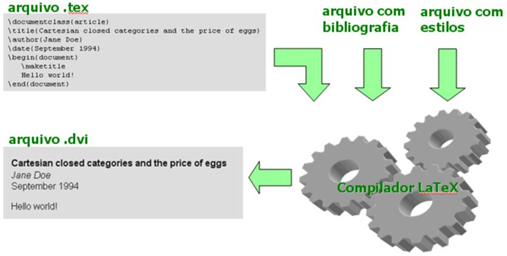
\includegraphics[scale=0.75]{Imagens/FiguraTeste.png}
  	\textsf{\caption{Teste de uma figura em formato .png}}
  	\label{fig:FiguraTeste}
\end{figure}


\section{Se��o 2}

Referenciamento da figura inserida na se��o anterior: \ref{fig:FiguraTeste}


\section{Se��o 3}

Se��o 3


\section{Se��o 4}

Se��o 4
	
	% Capitulo 3: Terceiro cap�tulo (arquivo Includes/Capitulo3.tex)
	% Cap�tulo 3
\chapter{Cap�tulo 3}

Algumas regras devem ser observadas na reda��o da disserta��o/tese: 

\begin{itemize}
   \item ser claro, preciso, direto, objetivo e conciso, utilizando frases curtas e evitando ordens inversas desnecess�rias;
   \item construir per�odos com no m�ximo duas ou tr�s linhas, bem como par�grafos com cinco linhas cheias, em m�dia, e no m�ximo oito (ou seja, n�o construir par�grafos e per�odos muito longos, pois isso cansa o(s) leitor(es) e pode fazer com que ele(s) percam a linha de racioc�nio desenvolvida);
   \item a simplicidade deve ser condi��o essencial do texto; a simplicidade do texto n�o implica necessariamente repeti��o de formas e frases desgastadas, uso exagerado de voz passiva (como \textit{ser� iniciado}, \textit{ser� realizado}), pobreza vocabular etc. Com palavras conhecidas de todos, � poss�vel escrever de maneira original e criativa e produzir frases elegantes, variadas, fluentes e bem alinhavadas;
   \item adotar como norma a ordem direta, por ser aquela que conduz mais facilmente o leitor � ess�ncia do texto, dispensando detalhes irrelevantes e indo diretamente ao que interessa, sem ``rodeios'' (verborragias);
   \item n�o come�ar per�odos ou par�grafos seguidos com a mesma palavra, nem usar repetidamente a mesma estrutura de frase;
   \item desprezar as longas descri��es e relatar o fato no menor n�mero poss�vel de palavras;
   \item recorrer aos termos t�cnicos somente quando absolutamente indispens�veis e nesse caso colocar o seu significado entre par�nteses (ou seja, n�o se deve admitir que todos os que ler�o o trabalho j� disp�em de algum conhecimento desenvolvido no mesmo);
   \item dispensar palavras e formas empoladas ou rebuscadas, que tentem transmitir ao leitor mera ideia de erudi��o (at� mesmo �s vezes ilus�ria);
   \item n�o perder de vista o universo vocabular do leitor, adotando a seguinte regra pr�tica: \textit{nunca escrever o que n�o se diria};
   \item termos coloquiais ou de g�ria devem ser usados com extrema parcim�nia (ou mesmo nem serem utilizados) e apenas em casos muito especiais, para n�o darem ao leitor a ideia de vulgaridade e descaracterizar o trabalho;
   \item ser rigoroso na escolha das palavras do texto, desconfiando dos sin�nimos perfeitos ou de termos que sirvam para todas as ocasi�es; em geral, h� uma palavra para definir uma situa��o;
   \item encadear o assunto de maneira suave e harmoniosa, evitando a cria��o de um texto onde os par�grafos se sucedem uns aos outros como compartimentos estanques, sem nenhuma flu�ncia entre si;
   \item ter um extremo cuidado durante a reda��o do texto, principalmente com rela��o �s regras gramaticais e ortogr�ficas da l�ngua; geralmente todo o texto � escrito na forma impessoal do verbo, n�o se utilizando, portanto, de termos em primeira pessoa, seja do plural ou do singular.
\end{itemize}

Continua��o do texto.


\section{Se��o 1}

Teste de tabela.

\begin{table}[!htb]
   \textsf{\caption{Tabela sem sentido.}}
   \centering
   \medskip
   \begin{tabular}{c|p{4cm}}
      \hline
      \textbf{T�tulo Coluna 1} & \textbf{T�tulo Coluna 2} \\
      \hline
      Texto curto & Texto mais extenso, que requer mais de uma linha \\
      \hline
      \label{tab:TabelaSemSentido}
   \end{tabular}
\end{table}


\section{Se��o 2}

Se��o 2


\subsection{Subse��o 2.1}

Refer�ncia � tabela definida no in�cio: \ref{tab:TabelaSemSentido}


\subsection{Subse��o 2.2}

Texto a ser enumerado.

\begin{enumerate}
   \item Item 1
   \item Item 2, com nota explicativa\footnote{Nota explicativa}
   \item Item 3
\end{enumerate}


\section{Se��o 3}

Texto antes de equa��o.

\begin{equation}
   x = y + z
\end{equation}

Texto depois de equa��o.
	
	% Capitulo 4: Quarto cap�tulo (arquivo Includes/Capitulo4.tex)
	% Cap�tulo 4
\chapter{Cap�tulo 4}

\section{Se��o 1}

Teste para s�mbolo

\simb[$\lambda$ (algum s�mbolo)]{$\lambda$}


\section{Se��o 2}

Teste para abreviatura 

\abrv[UFRN -- Universidade Federal do Rio Grande do Norte]{UFRN}

\abrv[DIMAp -- Departamento de Inform�tica e Matem�tica Aplicada]{DIMAp}

	
	% Capitulo 5: Quinto cap�tulo (arquivo Includes/Capitulo5.tex)
	% Cap�tulo 5
\chapter{Cap�tulo 5}

\section{Se��o 1}

Se��o 1


\section{Se��o 2}

Alguns exemplos de cita��o: 

Na tese de Doutorado de Paquete \cite{PaquetePhD}, discute-se sobre algoritmos de busca local estoc�sticos aplicados a problemas de Otimiza��o Combinat�ria considerando m�ltiplos objetivos. Por sua vez, o trabalho de \cite{KnowlesBoundedLebesgue}, publicado nos anais do IEEE CEC de 2003, mostra uma t�cnica de arquivamento tamb�m empregada no desenvolvimento de algoritmos evolucion�rios multi-objetivo, trabalho esse posteriormente estendido para um cap�tulo de livro dos mesmos autores \cite{KnowlesBoundedPareto}. Por fim, no relat�rio t�cnico de \citeonline{Jaszkiewicz}, fala-se sobre um algoritmo gen�tico h�brido para problemas multi-crit�rio, enquanto no artigo de jornal de Lopez \textit{et al.} \cite{LopezPaqueteStu} trata-se do \textit{trade-off} entre algoritmos gen�ticos e metodologias de busca local, tamb�m aplicados no contexto multi-crit�rio e relacionado de alguma forma ao trabalho de Jaszkiewicz (\citeyear{Jaszkiewicz}).

Outros exemplos relacionados encontram-se em \cite{Silberschatz} (livro), \cite{DB2XML} (refer�ncia da Web) e \cite{Angelo} (disserta��o de Mestrado).

\subsection{Subse��o 5.1}

Subse��o 5.1


\subsection{Subse��o 5.2}

Subsection 5.2


\section{Se��o 3}

Se��o 3
		
	% Consideracoes finais
	% Considera��es finais
\chapter{Considera��es finais}

As considera��es finais formam a parte final (fechamento) do texto, sendo dito de forma resumida (1) o que foi desenvolvido no presente trabalho e quais os resultados do mesmo, (2) o que se p�de concluir ap�s o desenvolvimento bem como as principais contribui��es do trabalho, e (3) perspectivas para o desenvolvimento de trabalhos futuros, como listado nos exemplos de se��o abaixo. O texto referente �s considera��es finais do autor deve salientar a extens�o e os resultados da contribui��o do trabalho e os argumentos utilizados estar baseados em dados comprovados e fundamentados nos resultados e na discuss�o do texto, contendo dedu��es l�gicas correspondentes aos objetivos do trabalho, propostos inicialmente.


\section{Principais contribui��es}

Texto.


\section{Limita��es}

Texto.


\section{Trabalhos futuros}

Texto.
	
	% Bibliografia (arquivo Capitulos/Referencias.bib)
	\bibliography{Capitulos/Referencias}
	\bibliographystyle{abnt-alf}
	
	% Ap�ndice A (arquivo Includes/ApendiceA)
	% Ap�ndice
\apendice
\chapter{Primeiro ap�ndice}

Os ap�ndices s�o textos ou documentos elaborados pelo autor, a fim de complementar sua argumenta��o, sem preju�zo da unidade nuclear do trabalho.
	
	% Anexo A (arquivo Includes/AnexoA)
	% Anexo
\anexo
\chapter{Primeiro anexo}

Os anexos s�o textos ou documentos n�o elaborado pelo autor, que servem de fundamenta��o, comprova��o e ilustra��o.
	
	% P�gina em branco
	\newpage

\end{document}